\chapter{Génomique et séquençage}\label{ch:b3:genomics}

Le premier génome complet d'un organisme vivant libre, les \qty{1.8}{Mb}
d'une bactérie, a été publié en 1995 après un an de travail d'une équipe
de quarante personnes. Le génome humain, \num{3.2} milliards de paires
de bases, a demandé treize ans et environ trois milliards de dollars à
un consortium international, et a été déclaré achevé en 2003.
Aujourd'hui une machine de paillasse lit un génome humain en une nuit
pour quelques centaines de dollars, un hôpital séquence la tumeur d'un
patient pour choisir un médicament, et un musée extrait et lit le génome
d'un os vieux de quarante mille ans. La technique qui a rendu cela
possible, les mathématiques qui transforment des millions de \omterm{def:b3:genomics:ngs}{lectures}
courtes en un génome, et ce que les génomes achevés ont appris sur la
taille, le contenu et l'histoire de notre ADN font l'objet de ce
chapitre. Le chapitre suivant reprend les algorithmes qui comparent les
séquences une fois qu'on les tient.

\section{Lire l'ADN}

\begin{definition}[Séquençage par terminaison de chaîne]\label{def:b3:genomics:sanger}
\index{séquençage de Sanger}\index{didésoxynucléotide}\index{terminaison de chaîne}
Le \emph{séquençage de Sanger} recopie une matrice simple brin à partir
d'une amorce, avec une ADN polymérase, en présence des quatre
nucléotides normaux et d'une petite proportion de
\emph{didésoxynucléotides}, dépourvus de l'hydroxyle 3$'$ et qui
terminent donc la chaîne partout où ils sont incorporés. Chaque
didésoxynucléotide porte un fluorophore différent. Le produit est un
mélange de fragments, un pour chaque position de la matrice, se
terminant chacun par une base d'identité connue~; séparés par la taille
dans un capillaire de gel, ils passent devant un détecteur par ordre de
longueur, et la suite des couleurs est la séquence de la matrice. Une
course lit \qtyrange{700}{900}{bp} avec un taux d'erreur inférieur à
$10^{-3}$~; elle reste la méthode pour vérifier une construction ou un
gène isolé.
\end{definition}

\begin{proof}[Faits expérimentaux]
Sanger, Nicklen et Coulson ont publié la méthode en 1977 et s'en sont
servis la même année pour lire les \qty{5386}{bp} du phage $\phi$X174
--- le premier génome d'ADN complet --- puis, en 1981, les
\qty{16569}{bp} de la mitochondrie humaine. Fleischmann et ses collègues
(1995) ont lu les \qty{1.83}{Mb} d'\emph{Haemophilus influenzae} en
brisant le génome entier en fragments aléatoires, en séquençant
\num{24000} d'entre eux et en assemblant les \omterm{def:b3:genomics:ngs}{lectures} par ordinateur ---
la stratégie du \emph{shotgun de génome entier} que tous les projets
ultérieurs ont amplifiée.
\end{proof}

\begin{omfigure}
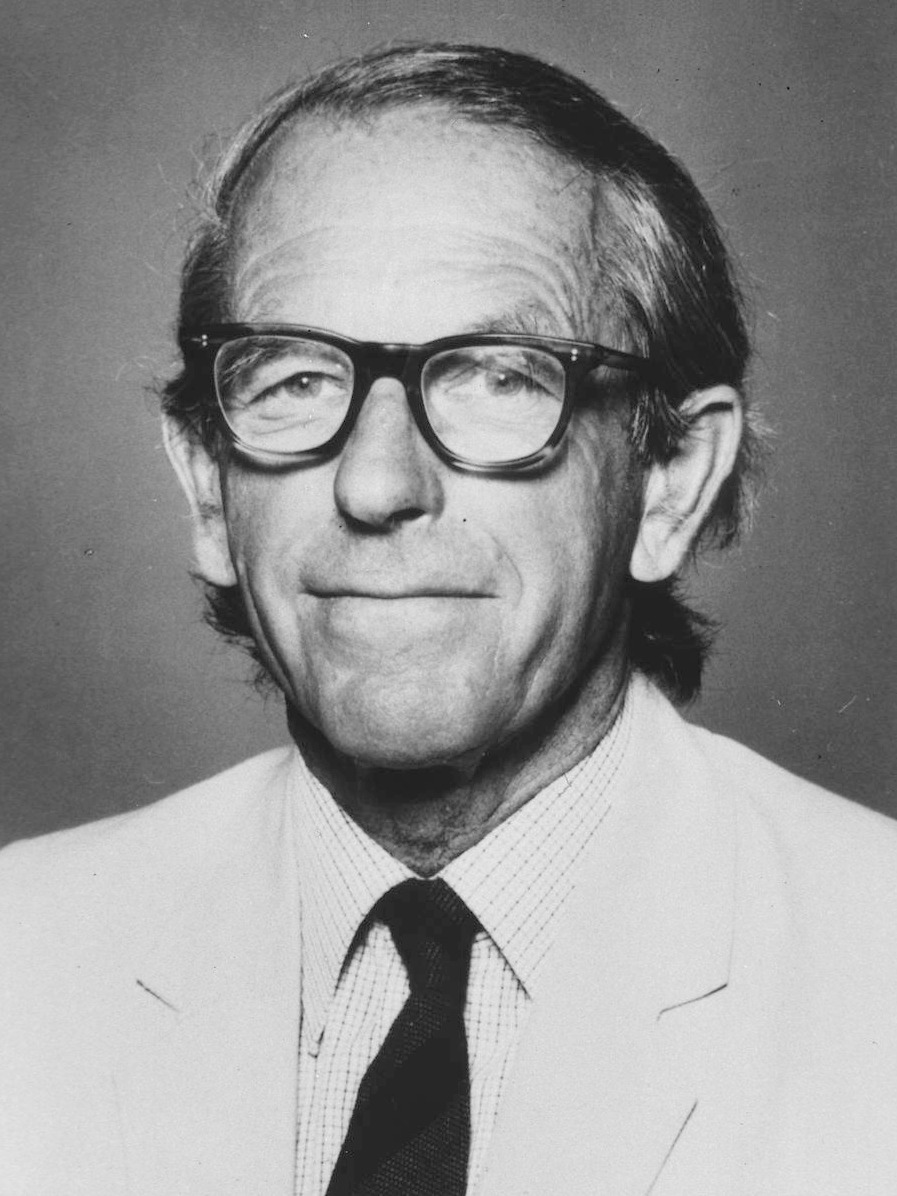
\includegraphics[width=0.30\linewidth]{images/book5/sanger.jpg}\hspace{0.04\linewidth}
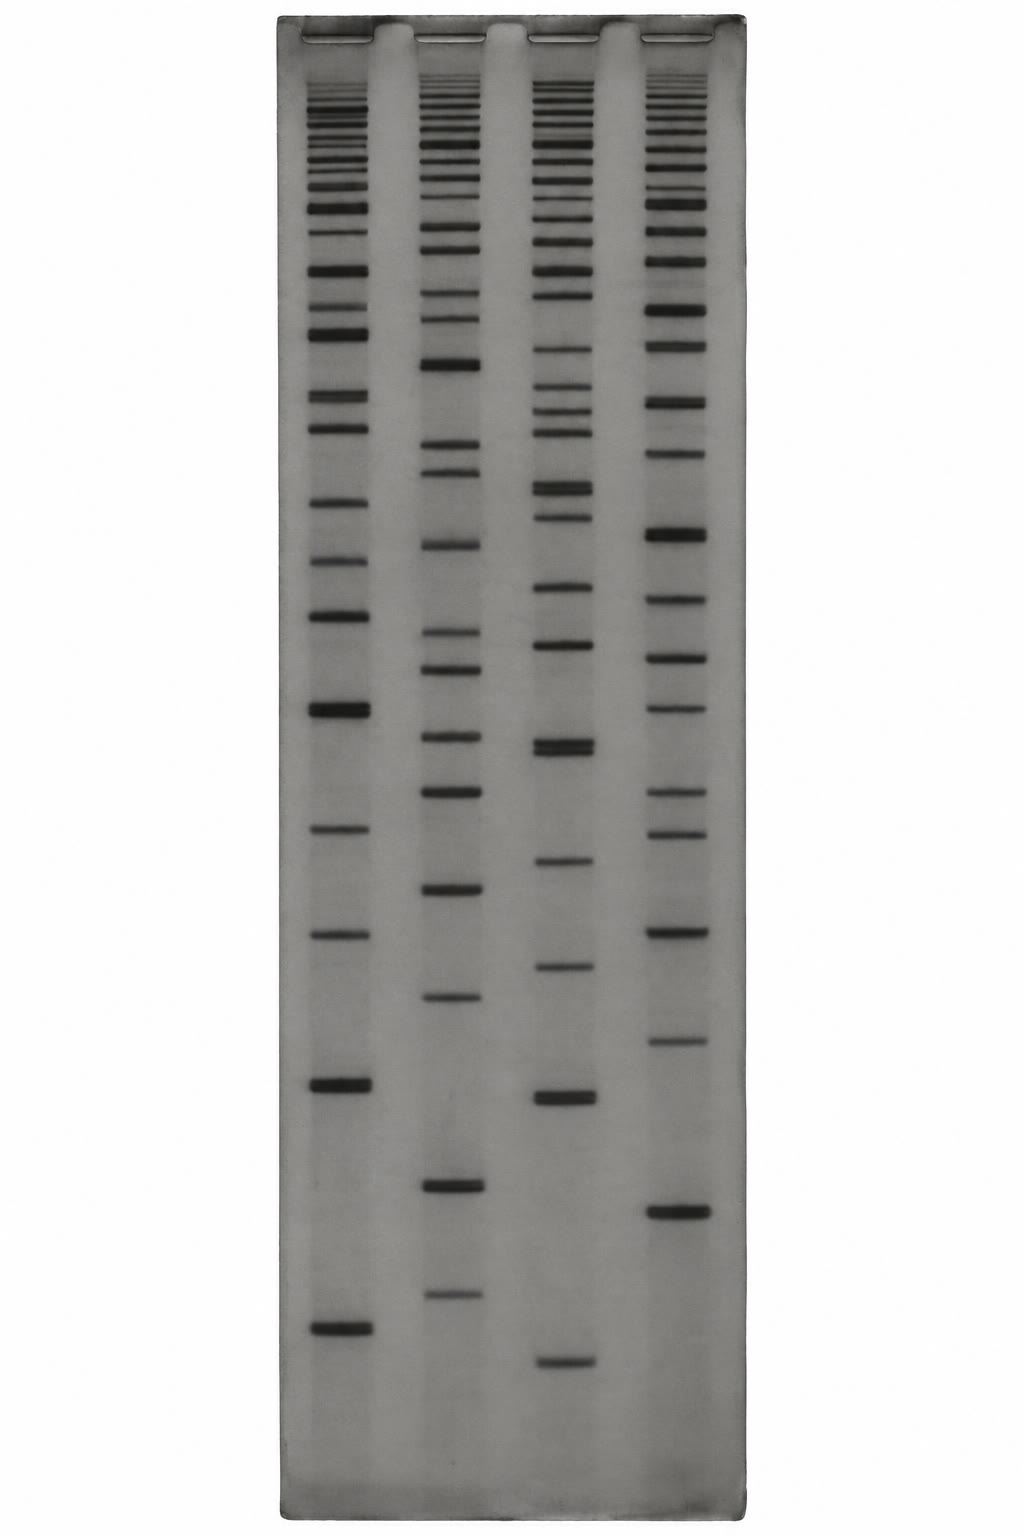
\includegraphics[width=0.30\linewidth]{images/book5/ai/b5-04-sanger-gel.jpg}

{\small À gauche~: Frederick Sanger, qui a mis au point les premières
méthodes praticables de \omterm{def:b3:genomics:ngs}{lecture} des protéines et de l'ADN et a reçu un
prix Nobel pour chacune. À droite~: l'autoradiographie d'un gel de
séquençage d'avant l'ère des capillaires, une piste par base, la
séquence se lisant de bas en haut sur l'échelle de bandes.}
\end{omfigure}

\begin{omfigure}
\begin{tikzpicture}[every node/.style={font=\scriptsize}, >=stealth]
  % template and primer
  \draw[very thick, omDef] (0,3.0) -- (6,3.0); \node[left] at (-0.1,3.0) {matrice 3$'$};
  \node[right] at (6.05,3.0) {5$'$};
  \foreach \x/\b in {0.6/T,1.2/G,1.8/A,2.4/C,3.0/T,3.6/T,4.2/G,4.8/C} \node[above, omDef] at (\x,3.05) {\b};
  \draw[very thick, omProp] (0,2.6) -- (0.3,2.6); \node[left] at (-0.1,2.6) {amorce};
  % terminated products
  \foreach \i/\len/\col/\b in {1/0.6/omDef/A, 2/1.2/omMeth/C, 3/1.8/omThm/T, 4/2.4/omExo/G, 5/3.0/omDef/A, 6/3.6/omDef/A, 7/4.2/omMeth/C, 8/4.8/omExo/G} {
    \draw[very thick, omProp] (0,2.6-0.32*\i) -- (\len-0.15,2.6-0.32*\i);
    \fill[\col] (\len-0.05,2.6-0.32*\i) circle (0.1);
    \node[right, \col] at (\len+0.05,2.6-0.32*\i) {dd\b};
  }
  \node[below, align=center] at (2.4,-0.25) {un produit pour chaque position, terminé chacun\\par une base didésoxy fluorescente};
  % capillary readout
  \draw[->, thick] (6.5,1.3) -- (7.4,1.3) node[midway, above] {taille};
  \draw[thick] (7.6,0.0) rectangle (11.6,2.6);
  \foreach \i/\col in {1/omDef, 2/omMeth, 3/omThm, 4/omExo, 5/omDef, 6/omDef, 7/omMeth, 8/omExo} {
    \draw[very thick, \col] (7.6+0.45*\i,0.1) .. controls (7.6+0.45*\i-0.15,0.1) and (7.6+0.45*\i-0.1,1.6) .. (7.6+0.45*\i,1.6) .. controls (7.6+0.45*\i+0.1,1.6) and (7.6+0.45*\i+0.15,0.1) .. (7.6+0.45*\i+0.3,0.1);
  }
  \foreach \i/\b in {1/A, 2/C, 3/T, 4/G, 5/A, 6/A, 7/C, 8/G} \node[above] at (7.6+0.45*\i,1.7) {\b};
  \node[below] at (9.6,-0.05) {la plus courte $\to$ la plus longue~: la séquence, lue en couleurs};
\end{tikzpicture}

{\small Séquençage par \omterm{def:b3:genomics:sanger}{terminaison de chaîne}. Une base didésoxy achève
la copie à chaque position où elle est incorporée~; les fragments, un
par longueur, sont séparés par la taille et la couleur de chaque base
terminale se lit dans l'ordre.}
\end{omfigure}

\begin{definition}[Séquençage massivement parallèle]\label{def:b3:genomics:ngs}
\index{séquençage par synthèse}\index{lecture}\index{séquençage à longues lectures}\index{nanopore}
Les instruments de deuxième génération lisent des millions à des
milliards de fragments à la fois. Dans le \emph{séquençage par
synthèse}, les fragments, munis d'adaptateurs ligaturés à leurs
extrémités, sont fixés sur une cellule de verre et amplifiés sur place
en amas de molécules identiques~; les amas sont ensuite allongés d'une
base par cycle avec des nucléotides fluorescents et réversiblement
bloqués, imagés, débloqués, puis allongés de nouveau, de sorte que
chaque cycle ajoute une base à la \emph{lecture} de chaque amas. Les
lectures font \qtyrange{100}{300}{bp}, le plus souvent depuis les deux
extrémités d'un fragment (\emph{extrémités appariées}), avec un taux
d'erreur d'environ $10^{-3}$ par base, et une course livre jusqu'à
$10^{12}$ bases. Les instruments de troisième génération, à
\emph{longues lectures}, lisent des molécules uniques sans
amplification~: en regardant une polymérase incorporer en temps réel des
nucléotides fluorescents, ou en faisant passer l'ADN par un
\emph{nanopore} protéique et en enregistrant le courant ionique, que
chaque suite de bases module à sa façon. Des lectures de
\qtyrange{10}{100}{kb} et davantage franchissent les répétitions que les
lectures courtes ne franchissent pas, au prix d'un taux d'erreur brut
plus élevé que le consensus réduit.
\end{definition}

\begin{omfigure}
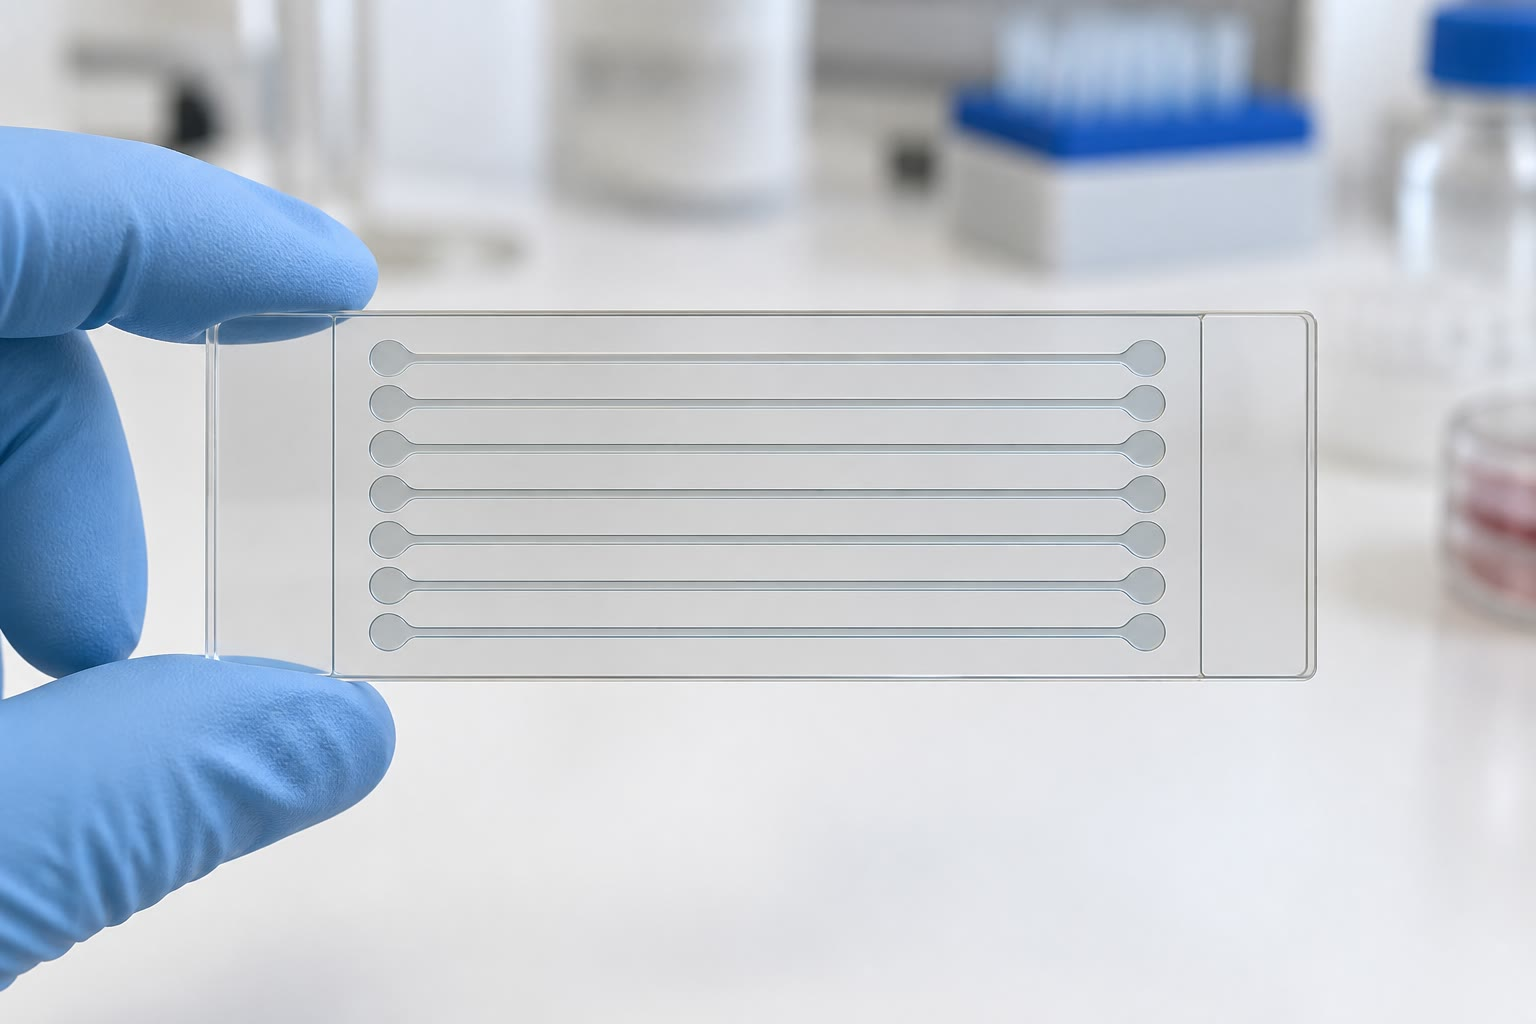
\includegraphics[width=0.46\linewidth]{images/book5/ai/b5-04-flowcell.jpg}\hspace{0.04\linewidth}

\includegraphics[width=0.46\linewidth]{images/book5/ai/b5-04-nanopore.jpg}

{\small À gauche~: une cellule de flux, la lame de verre sur laquelle
des milliards d'amas d'ADN sont cultivés et lus une base par cycle. À
droite~: un séquenceur à \omterm{def:b3:genomics:ngs}{nanopores} de poche, qui lit des molécules
uniques sous forme de variations d'un courant ionique.}
\end{omfigure}

\begin{theorem}[Couverture et lacunes d'un projet shotgun]\label{thm:b3:genomics:lander-waterman}
\index{couverture}\index{Lander--Waterman}\index{contig}
Soit $N$ \omterm{def:b3:genomics:ngs}{lectures} de longueur $L$ prises à des positions aléatoires le
long d'un génome de longueur $G$, et soit $c = NL/G$ la
\emph{couverture}, nombre moyen de \omterm{def:b3:genomics:ngs}{lectures} couvrant une base. Une base
donnée est alors couverte par un nombre de \omterm{def:b3:genomics:ngs}{lectures} qui suit une loi de
Poisson de moyenne $c$~: la fraction du génome laissée non séquencée
vaut
\[
P(\text{non couvert}) = e^{-c},
\]
et si l'on ne reconnaît deux \omterm{def:b3:genomics:ngs}{lectures} comme chevauchantes que
lorsqu'elles partagent au moins $T$ bases, en posant $\theta = T/L$, le
nombre espéré de \emph{contigs} (îlots de \omterm{def:b3:genomics:ngs}{lectures} chevauchantes) vaut
\[
\text{contigs} = N\,e^{-c(1-\theta)},
\]
et leur longueur moyenne vaut à peu près
$L\,\bigl(e^{c(1-\theta)} - 1\bigr)/c + L\theta$.
\end{theorem}
\begin{proof}
Les points de départ des \omterm{def:b3:genomics:ngs}{lectures} tombent au hasard avec la densité
$N/G$ par base. Une base est couverte par les \omterm{def:b3:genomics:ngs}{lectures} qui commencent
dans les $L$ bases qui la précèdent~; le nombre de départs dans une
fenêtre de longueur $L$ suit une loi de Poisson de moyenne $LN/G
= c$, et la probabilité qu'il n'y en ait aucun vaut $e^{-c}$. Une
\omterm{def:b3:genomics:ngs}{lecture} est la plus à droite de son contig si aucune autre \omterm{def:b3:genomics:ngs}{lecture} ne
commence dans les $L - T = L(1-\theta)$ bases qui suivent son propre
départ (une \omterm{def:b3:genomics:ngs}{lecture} commençant plus tard la chevaucherait de moins de
$T$ et ne serait pas jointe)~; cette probabilité vaut
$e^{-c(1-\theta)}$, et comme chaque contig a exactement une \omterm{def:b3:genomics:ngs}{lecture} la
plus à droite, le nombre espéré de contigs vaut $N e^{-c(1-\theta)}$.
La longueur moyenne d'un contig s'obtient en divisant $G$ par le nombre
de contigs, corrigé de la fraction non couverte.
\end{proof}

\begin{example}[Combien suffit]\label{ex:b3:genomics:coverage}
À $c = 5$ la fraction non séquencée vaut $e^{-5} = 0.7\,\%$ --- pour un
génome de \qty{3.2}{Gb}, vingt millions de bases réparties en quelques
dizaines de milliers de lacunes. À $c = 10$ elle vaut
$4.5\times 10^{-5}$, soit \qty{150}{kb} en tout. Les génomes humains
sont couramment séquencés à $c = 30$, non pas à cause des lacunes de
couverture ($e^{-30} \approx 10^{-13}$), mais parce que chaque base
doit être lue plusieurs fois sur chacun des deux chromosomes pour
appeler un variant hétérozygote avec confiance contre un taux d'erreur
de $10^{-3}$ par \omterm{def:b3:genomics:ngs}{lecture}. Les génomes bactériens sont séquencés à
$c = 50$--$100$ pour la même raison et parce que c'est bon marché. La
formule montre aussi ce que la couverture ne peut pas réparer~: une
répétition plus longue qu'une \omterm{def:b3:genomics:ngs}{lecture} est un endroit où le graphe de
chevauchement se ramifie, et aucune quantité de \omterm{def:b3:genomics:ngs}{lectures} courtes ne la
résout. C'est à cela que servent les longues \omterm{def:b3:genomics:ngs}{lectures}.
\end{example}

\begin{omfigure}
\begin{tikzpicture}
\begin{axis}[
  width=0.7\linewidth, height=5.6cm,
  axis x line=bottom, axis y line=left,
  xmin=0, xmax=12, ymin=0.000001, ymax=1, ymode=log,
  xlabel={couverture $c$}, ylabel={fraction},
  xlabel style={font=\small, at={(axis description cs:0.5,-0.12)}, anchor=north},
  ylabel style={font=\small},
  tick label style={font=\small}, xtick={0,2,4,6,8,10,12},
  clip=false,
]
\addplot[very thick, omDef, domain=0:12, samples=40] {exp(-x)};
\addplot[very thick, omThm, domain=0.3:12, samples=40] {exp(-x*0.8)*x/12};
\node[font=\scriptsize, omDef, anchor=north west] at (axis cs:0.3,0.002) {fraction non couverte $e^{-c}$};
\node[font=\scriptsize, omThm, anchor=south west] at (axis cs:5.5,0.03) {contigs par lecture $\times\, c/12$, $\theta = 0.2$};
\end{axis}
\end{tikzpicture}

{\small Les deux quantités de Lander--Waterman en fonction de la
couverture~: la fraction du génome jamais lue décroît en $e^{-c}$, et le
nombre de contigs (ici rapporté à une \omterm{def:b3:genomics:ngs}{lecture}) passe par un maximum à
faible couverture puis décroît à mesure que les îlots fusionnent.}
\end{omfigure}

\section{Des lectures au génome}

\begin{definition}[Assemblage et annotation]\label{def:b3:genomics:assembly}
\index{assemblage}\index{échafaudage}\index{N50}\index{annotation}\index{génome de référence}
L'\emph{assemblage} reconstitue un génome à partir de ses \omterm{def:b3:genomics:ngs}{lectures} par
chevauchement~: dans un \emph{graphe de chevauchement}, chaque \omterm{def:b3:genomics:ngs}{lecture}
est un sommet relié aux \omterm{def:b3:genomics:ngs}{lectures} qu'elle chevauche~; dans un
\emph{graphe de de Bruijn}, employé pour des milliards de \omterm{def:b3:genomics:ngs}{lectures}
courtes, chaque $k$-mer (sous-séquence de longueur $k$) est un sommet et
le génome est un chemin qui les parcourt. Les deux sont brisés par les
répétitions plus longues que la \omterm{def:b3:genomics:ngs}{lecture}, qui donnent des chemins
ramifiés. Les contigs sont ordonnés et orientés en \emph{échafaudages}
grâce aux \omterm{def:b3:genomics:ngs}{lectures} à extrémités appariées et à des informations à longue
portée (longues \omterm{def:b3:genomics:ngs}{lectures}, cartes optiques, cartes de contacts
chromosomiques), et les échafaudages sont placés sur les chromosomes. La
qualité d'un assemblage se résume par le \emph{N50}~: la longueur de
contig telle que la moitié des bases assemblées se trouve dans des
contigs au moins aussi longs. L'\emph{annotation} cherche ensuite les
gènes~: chez les bactéries, les cadres de \omterm{def:b3:genomics:ngs}{lecture} ouverts plus longs que
le hasard ne le veut~; chez les eucaryotes, en combinant des signaux de
séquence (sites d'épissage, promoteurs, usage des codons), l'homologie
avec des protéines connues et des transcrits séquencés à partir de
l'ARN. Le résultat, pour une espèce, est un \emph{génome de référence}
sur lequel toute \omterm{def:b3:genomics:ngs}{lecture} ultérieure de cette espèce est alignée plutôt
que réassemblée.
\end{definition}

\begin{method}[D'un échantillon aux variants]\label{met:b3:genomics:pipeline}
\index{appel de variants}
Pour une étude de reséquençage d'un individu contre une référence~:
(1) extraire l'ADN, le fragmenter à \qtyrange{300}{500}{bp}, ligaturer
des adaptateurs (la \emph{banque})~; (2) séquencer à la couverture
voulue (30$\times$ pour un génome humain, 100$\times$ pour un exome, qui
capture les \qty{1.5}{\%} du génome qui codent une protéine)~;
(3) aligner chaque \omterm{def:b3:genomics:ngs}{lecture} sur la référence, en tolérant des
mésappariements~; (4) à chaque position, compter les bases dans les
\omterm{def:b3:genomics:ngs}{lectures}~: une position où la moitié environ des \omterm{def:b3:genomics:ngs}{lectures} s'écarte de la
référence est un \emph{variant} hétérozygote, une position où presque
toutes s'en écartent un variant homozygote, une position où quelques-unes
seulement s'en écartent une erreur~; (5) filtrer sur la profondeur, la
qualité des bases et l'équilibre entre brins~; (6) annoter chaque
variant par son effet sur les gènes (synonyme, faux-sens, non-sens,
épissage, décalage du cadre) et par sa fréquence dans les bases de
données de populations~; (7) pour un diagnostic, garder les variants
rares prédits délétères dans des gènes compatibles avec le phénotype, et
confirmer par un \omterm{def:b3:genomics:sanger}{séquençage de Sanger}.
\end{method}

\section{À quoi ressemblent les génomes}

\begin{proposition}[Taille du génome et nombre de gènes]\label{prop:b3:genomics:sizes}
\index{paradoxe de la valeur C}\index{taille du génome}
Les tailles de génome couvrent un facteur $10^{5}$ chez les eucaryotes
--- \qty{12}{Mb} pour la levure, \qty{100}{Mb} pour le ver,
\qty{140}{Mb} pour la mouche, \qty{3.2}{Gb} pour l'homme, \qty{16}{Gb}
pour l'oignon, \qty{130}{Gb} pour un dipneuste, \qty{150}{Gb} pour le
lis \emph{Paris japonica} --- alors que les nombres de gènes couvrent à
peine un facteur $10$~: \num{6000} chez la levure, \num{20000} chez le
ver, \num{14000} chez la mouche, environ \num{20000} gènes codants chez
l'homme, \num{40000} chez le riz. C'est le \emph{paradoxe de la valeur
C}~: la \omterm{prop:b3:genomics:sizes}{taille du génome} ne mesure pas la complexité, et le nombre de
gènes non plus. Ce qui varie est le contenu non codant --- introns,
éléments transposables, répétitions satellites --- et le nombre de
protéines qu'un génome peut produire est multiplié bien au-delà de son
nombre de gènes par l'épissage alternatif
(\cref{ch:b3:rna-regulation}) et par la régulation, où s'écrit
l'essentiel de la complexité d'un organisme. Les génomes bactériens,
eux, sont compacts et leur taille suit bien le nombre de gènes~: environ
un gène par kilobase, \qty{88}{\%} de codant chez \emph{E.~coli}.
\end{proposition}

\begin{example}[Le génome humain par son contenu]\label{ex:b3:genomics:content}
Sur les \qty{3.2}{Gb}~: exons codants, \qty{1.5}{\%}~; introns et régions
non traduites des gènes, environ \qty{35}{\%}~; éléments transposables
et leurs fossiles, environ \qty{45}{\%} --- rétrotransposons LINE-1
\qty{17}{\%}, éléments Alu \qty{10}{\%} (plus d'un million de copies
d'une séquence de \qty{300}{bp}), rétrovirus endogènes \qty{8}{\%}~;
duplications segmentaires \qty{5}{\%}~; répétitions simples et
satellites, y compris les centromères, environ \qty{5}{\%}~; le reste en
séquence unique non codante, où vivent les éléments régulateurs. Quelque
\numrange{100}{200} gènes codent encore une machinerie LINE-1 active, et
de nouvelles insertions surviennent à peu près une naissance sur vingt.
Environ \qty{8}{\%} du génome est sous sélection purificatrice
détectable --- bien plus que les exons --- et l'essentiel de cela est
régulateur.
\end{example}

\begin{omfigure}
\begin{tikzpicture}[every node/.style={font=\scriptsize}]
  \def\w{12}
  % stacked bar: fractions
  \fill[omThm] (0,0) rectangle (0.18,0.7);
  \fill[omDef!60] (0.18,0) rectangle (4.38,0.7);
  \fill[omProp!70] (4.38,0) rectangle (6.42,0.7);
  \fill[omProp!45] (6.42,0) rectangle (7.62,0.7);
  \fill[omProp!25] (7.62,0) rectangle (9.78,0.7);
  \fill[omMeth!50] (9.78,0) rectangle (10.38,0.7);
  \fill[gray!45] (10.38,0) rectangle (10.98,0.7);
  \fill[gray!15] (10.98,0) rectangle (12,0.7);
  \draw[thick] (0,0) rectangle (12,0.7);
  % labels above/below with leaders
  \draw (0.09,0.7) -- (0.09,1.1); \node[above, align=center] at (0.5,1.1) {exons\\\qty{1.5}{\%}};
  \node[above] at (2.3,0.75) {introns, UTR des gènes~: \qty{35}{\%}};
  \node[below, align=center] at (5.4,-0.05) {LINE-1\\\qty{17}{\%}};
  \node[below, align=center] at (7.0,-0.05) {Alu\\\qty{10}{\%}};
  \node[below, align=center] at (8.7,-0.05) {autres transposons,\\rétrovirus \qty{18}{\%}};
  \node[above, align=center] at (10.1,0.75) {duplications\\segmentaires \qty{5}{\%}};
  \node[below, align=center] at (10.7,-0.05) {satellites\\\qty{5}{\%}};
  \draw[gray] (11.5,0.72) -- (12.0,1.05); \node[above, align=center] at (12.3,1.05) {autre séquence\\unique non codante};
  \draw[decorate, decoration={brace, amplitude=4pt, mirror}] (4.38,-1.0) -- (9.78,-1.0) node[midway, below=4pt] {issu d'éléments transposables~: \qty{45}{\%}};
\end{tikzpicture}

{\small Le génome humain par son contenu, à l'échelle. Les exons codants
(rouge) n'en sont qu'un filet~; près de la moitié du génome descend
d'éléments transposables.}
\end{omfigure}

\begin{definition}[Génomique comparée]\label{def:b3:genomics:comparative}
\index{orthologue}\index{paralogue}\index{synténie}\index{élément non codant conservé}\index{duplication du génome entier}
Des gènes de deux espèces descendus d'un même gène de leur ancêtre
commun sont \emph{orthologues}~; des gènes d'une même espèce descendus
d'une duplication sont \emph{paralogues}. Les blocs de chromosome où
l'ordre des gènes est conservé entre espèces sont dits
\emph{synténiques}~; la synténie permet de localiser un gène dans un
génome à partir de sa position dans un autre et révèle les remaniements
qui séparent deux caryotypes (environ \num{1000} entre l'homme et la
souris). Les séquences conservées entre espèces éloignées et qui ne
codent aucune protéine --- les \emph{éléments non codants conservés},
dont certains sont ultraconservés à la base près sur \qty{200}{bp}
entre l'homme et le poisson --- sont pour la plupart des amplificateurs
de gènes du développement. Des \emph{duplications du génome entier} ont
marqué l'histoire de certaines lignées~: deux tours à l'origine des
vertébrés (les quatre complexes Hox des mammifères contre l'unique
complexe des invertébrés), un chez l'ancêtre des salmonidés, un dans la
lignée des levures, plusieurs chez les plantes à fleurs~; les gènes
dupliqués sont pour la plupart perdus en quelques dizaines de millions
d'années, et les survivants divergent par leur fonction.
\end{definition}

\begin{example}[L'homme et le chimpanzé]\label{ex:b3:genomics:chimp}
Les séquences en copie unique alignées diffèrent entre l'homme et le
chimpanzé sur \qty{1.2}{\%} des bases --- quelque \num{35} millions de
substitutions --- et par des insertions et des délétions qui totalisent
encore \qty{3}{\%} de chaque génome. Deux humains diffèrent à raison
d'environ une base sur mille, soit quelque \numrange{4}{5} millions de
sites, plus quelques milliers de variants structuraux~; deux
chimpanzés, dont la population est plus grande depuis plus longtemps,
un peu davantage. Un enfant porte environ \num{70} mutations nouvelles
absentes de ses deux parents, dont les quatre cinquièmes viennent du
père, et ce nombre croît d'environ deux par année d'âge paternel ---
l'arithmétique du \cref{ch:b3:dna-repair} appliquée aux nombreuses
divisions de la spermatogenèse.
\end{example}

\section{Génomes et caractères}

\begin{definition}[Association pangénomique]\label{def:b3:genomics:gwas}
\index{étude d'association pangénomique}\index{polymorphisme nucléotidique}\index{score polygénique}
Un \emph{polymorphisme nucléotidique} (SNP) est une position où deux
bases apparaissent chacune chez au moins \qty{1}{\%} d'une population~;
une dizaine de millions sont fréquents chez l'homme. Une \emph{étude
d'association pangénomique} (GWAS) génotype des centaines de milliers de
SNP chez des milliers de personnes atteintes d'une maladie et des
milliers d'indemnes, et demande à chaque SNP si un allèle est plus
fréquent chez les cas. Comme un million de tests sont faits, un résultat
ne compte qu'en deçà d'un seuil de signification voisin de
$5\times 10^{-8}$ ($0.05$ divisé par le million de tests effectivement
indépendants). Les SNP associés marquent une région et non un variant
causal, puisque les allèles voisins voyagent ensemble (déséquilibre de
liaison) sur des dizaines de kilobases. Pour la plupart des maladies
fréquentes, chacun des allèles associés déplace le risque de quelques
pour cent et se trouve le plus souvent en séquence régulatrice~; leur
effet combiné, sommé sur des milliers de SNP en un \emph{score
polygénique}, explique une fraction de l'héritabilité et prédit le
risque à peu près aussi bien que l'histoire familiale.
\end{definition}

\begin{remark}[Ce que la génomique a tenu et n'a pas tenu]\label{rem:b3:genomics:delivered}
Le séquençage a été décisif là où un seul gène a un grand effet~:
plusieurs milliers de maladies mendéliennes ont leur gène, et séquencer
l'exome d'un enfant atteint d'un trouble non diagnostiqué donne un
diagnostic dans un tiers des cas environ. Les génomes de tumeurs
révèlent quels moteurs une tumeur porte et quels médicaments peuvent
agir (\cref{ch:b3:cancer-biology})~; les génomes de pathogènes retracent
les épidémies souche par souche (\cref{ch:b3:bacteriology})~; les
génomes anciens ont réécrit la préhistoire humaine, en montrant que les
populations hors d'Afrique portent environ \qty{2}{\%} d'ADN de
Néandertal. Pour les maladies fréquentes --- diabète, maladies
cardiaques, schizophrénie --- la génomique a livré des milliers de
petits effets et peu de mécanismes, et la promesse d'une prédiction à
partir du génome d'une personne en bonne santé reste modeste. Le génome
est une liste de pièces~; la biologie de leurs interactions ne s'y lit
pas.
\end{remark}

\section{Exercices}

\begin{exercise}[$\star$]\label{exo:b3:genomics:1}
Expliquer pourquoi un \omterm{def:b3:genomics:sanger}{didésoxynucléotide} termine une chaîne d'ADN en
croissance, et pourquoi une réaction de Sanger doit contenir à la fois
la forme normale et la forme didésoxy de chaque nucléotide.
\end{exercise}

\begin{exercise}[$\star$]\label{exo:b3:genomics:2}
Une course produit $4\times 10^{8}$ \omterm{def:b3:genomics:ngs}{lectures} appariées de
$2\times \qty{150}{bp}$. Quelle couverture cela donne-t-il d'un génome
humain de \qty{3.2}{Gb}~? Et d'un génome bactérien de \qty{5}{Mb}~?
\end{exercise}

\begin{exercise}[$\star$]\label{exo:b3:genomics:3}
Définir contig, \omterm{def:b3:genomics:assembly}{échafaudage} et \omterm{def:b3:genomics:assembly}{N50}. Un \omterm{def:b3:genomics:assembly}{assemblage} de \qty{100}{Mb}
compte dix contigs de \qty{8}{Mb} et \num{2000} de \qty{10}{kb}. Quel
est son \omterm{def:b3:genomics:assembly}{N50}~?
\end{exercise}

\begin{exercise}[$\star$]\label{exo:b3:genomics:4}
Énoncer le paradoxe de la valeur C avec deux exemples, et dire ce qui
explique surtout l'ADN en excès des grands génomes.
\end{exercise}

\begin{exercise}[$\star\star$]\label{exo:b3:genomics:5}
À l'aide du \cref{thm:b3:genomics:lander-waterman}, trouver la
couverture nécessaire pour ne laisser au plus qu'une base sur un million
non séquencée, et le nombre espéré de contigs pour un génome de
\qty{5}{Mb} lu à $c = 8$ avec des \omterm{def:b3:genomics:ngs}{lectures} de \qty{150}{bp} et un
chevauchement minimal de \qty{30}{bp}.
\end{exercise}

\begin{exercise}[$\star\star$]\label{exo:b3:genomics:6}
Un variant hétérozygote est couvert par $30$ \omterm{def:b3:genomics:ngs}{lectures}. En supposant que
chaque \omterm{def:b3:genomics:ngs}{lecture} montre l'un ou l'autre allèle avec la probabilité $1/2$,
quelle est la probabilité que moins de $8$ \omterm{def:b3:genomics:ngs}{lectures} montrent l'allèle
variant (au point qu'on puisse le prendre pour des erreurs)~? Utiliser
une approximation normale de moyenne $15$ et d'écart type $\sqrt{7.5}$.
Pourquoi $30\times$ est-il la norme~?
\end{exercise}

\begin{exercise}[$\star\star$]\label{exo:b3:genomics:7}
Un génome contient une répétition de \qty{6}{kb} présente en \num{500}
copies. Expliquer pourquoi un \omterm{def:b3:genomics:assembly}{assemblage} à partir de \omterm{def:b3:genomics:ngs}{lectures} de
\qty{150}{bp} l'effondre, à quoi ressemble le graphe obtenu, et quelle
longueur de \omterm{def:b3:genomics:ngs}{lecture} la résoudrait.
\end{exercise}

\begin{exercise}[$\star\star$]\label{exo:b3:genomics:8}
Deux humains diffèrent à raison d'une base sur mille. Combien de
différences dans leurs exomes (\qty{48}{Mb} de séquence codante)~? Si
les deux tiers des différences codantes sont synonymes ou bénignes et
que le reste modifie une protéine, combien de variants modifiant une
protéine une personne porte-t-elle par rapport à une autre~?
\end{exercise}

\begin{exercise}[$\star\star$]\label{exo:b3:genomics:9}
Une GWAS teste $10^{6}$ SNP au seuil $p < 5\times 10^{-8}$. Combien de
faux positifs attend-on si aucun SNP n'est réellement associé~? Un
allèle d'un SNP fait passer le risque d'une maladie de fréquence
\qty{2}{\%} à \qty{2.3}{\%}. Expliquer pourquoi un tel effet est
indétectable dans une étude de mille personnes et inutile pour un
individu, et pourquoi il peut néanmoins désigner un mécanisme.
\end{exercise}

\begin{exercise}[$\star\star\star$]\label{exo:b3:genomics:10}
Les génomes bactériens sont codants à \qty{88}{\%}, le génome humain à
\qty{1.5}{\%}. Donner trois hypothèses --- de génétique des populations,
structurale et régulatrice --- pour expliquer cette différence, et pour
chacune une observation génomique qui l'étaie ou la mine.
\end{exercise}

\begin{exercise}[$\star\star\star$]\label{exo:b3:genomics:11}
Établir le nombre de contigs de Lander--Waterman pour un mélange de
\omterm{def:b3:genomics:ngs}{lectures} de deux longueurs~: $N_{1}$ \omterm{def:b3:genomics:ngs}{lectures} courtes de longueur
$L_{1}$ et $N_{2}$ \omterm{def:b3:genomics:ngs}{lectures} longues de longueur $L_{2}$, les
chevauchements étant comptés avec le même minimum $T$. (Traiter chaque
\omterm{def:b3:genomics:ngs}{lecture} comme la plus à droite de son contig si aucune \omterm{def:b3:genomics:ngs}{lecture}, de l'une
ou l'autre sorte, ne commence dans sa propre longueur moins $T$.)
Montrer que quelques longues \omterm{def:b3:genomics:ngs}{lectures} réduisent le nombre de contigs
plus qu'un même nombre de bases en \omterm{def:b3:genomics:ngs}{lectures} courtes.
\end{exercise}

\begin{exercise}[$\star\star\star$]\label{exo:b3:genomics:12}
On soutient que les quatre complexes Hox des mammifères descendent d'un
seul complexe par deux tours de \omterm{def:b3:genomics:comparative}{duplication du génome entier} à la base
des vertébrés. Dire quelle configuration de \omterm{def:b3:genomics:comparative}{paralogues} à l'échelle du
génome, et quelle configuration dans les génomes des lamproies et des
cordés invertébrés, cette hypothèse prédit, et comment on la
distinguerait de deux duplications indépendantes du seul complexe.
\end{exercise}

\section{Problème~: deux génomes sur une même machine}

\begin{problem}[{Problème du week-end --- une bactérie et un homme
séquencés sur la même course~: les lectures réparties, la couverture et
les lacunes calculées, les contigs dénombrés, les variants hétérozygotes
appelés contre le taux d'erreur, le contenu du génome humain pesé et une
étude d'association dimensionnée, pour finir sur le nombre de contigs à
faible couverture, la couverture qui rend sûr l'appel d'un variant et le
nombre de mutations nouvelles chez un enfant}]
\label{pb:b3:genomics:1}
Données~: une course livre $6\times 10^{8}$ \omterm{def:b3:genomics:ngs}{lectures} de \qty{150}{bp}.
Un génome bactérien fait \qty{4.6}{Mb}~; le génome humain \qty{3.2}{Gb}
(haploïde). Chevauchement minimal $T = \qty{30}{bp}$. Taux d'erreur
$10^{-3}$ par base et par \omterm{def:b3:genomics:ngs}{lecture}. Séquence codante humaine
\qty{48}{Mb}~; le génome est issu à \qty{45}{\%} de transposons, avec
$1.1$ million de copies d'Alu de \qty{300}{bp}. Deux humains diffèrent
sur un site sur \num{1000}. Taux de mutation $1.2\times 10^{-8}$ par
base et par génération.

\medskip
\noindent\textbf{Partie I --- La bactérie.}
\begin{enumerate}
  \item On donne à la bactérie \qty{0.2}{\%} de la course. Combien de
        \omterm{def:b3:genomics:ngs}{lectures}, et quelle couverture~?
  \item Quelle fraction de son génome n'est pas séquencée~? Combien de
        bases cela fait-il~?
  \item Calculer $\theta$ et le nombre espéré de contigs.
  \item Un essai antérieur n'utilisait que \num{30000} \omterm{def:b3:genomics:ngs}{lectures}.
        Couverture, fraction non couverte et nombre de contigs~?
  \item Le génome contient \num{7} copies d'un opéron d'ARN
        ribosomique de \qty{5}{kb}. Expliquer ce qu'elles deviennent
        dans l'\omterm{def:b3:genomics:assembly}{assemblage} et combien d'extrémités de contigs cela seul
        produit.
  \item La bactérie a environ un gène par kilobase. Combien de gènes
        et, si \qty{88}{\%} du génome est codant, quelle est la
        longueur moyenne d'un gène~?
\end{enumerate}

\medskip
\noindent\textbf{Partie II --- L'homme.}
\begin{enumerate}[resume]
  \item Le reste de la course va à un seul génome humain. Quelle
        couverture du génome diploïde par copie haploïde (c'est-à-dire
        le nombre total de bases divisé par \qty{3.2}{Gb})~?
  \item À un site hétérozygote, chacun des deux allèles est couvert par
        la moitié environ des \omterm{def:b3:genomics:ngs}{lectures}. Avec la couverture de la
        question 7, quel est le nombre attendu de \omterm{def:b3:genomics:ngs}{lectures} montrant
        chaque allèle~?
  \item Une erreur fait apparaître une base fausse dans une \omterm{def:b3:genomics:ngs}{lecture}
        avec la probabilité $10^{-3}$. À un site homozygote couvert par
        $c$ \omterm{def:b3:genomics:ngs}{lectures}, quel est le nombre attendu de \omterm{def:b3:genomics:ngs}{lectures} montrant
        une base fausse donnée ($10^{-3}/3$ chacune)~? Pourquoi une
        règle «~appeler un variant si au moins $3$ \omterm{def:b3:genomics:ngs}{lectures} et au moins
        \qty{20}{\%} des \omterm{def:b3:genomics:ngs}{lectures} le montrent~» rejette-t-elle les
        erreurs à cette couverture~?
  \item Combien de sites hétérozygotes un humain porte-t-il (la moitié
        environ des différences entre deux génomes pris au hasard se
        trouvent dans chacun~; prendre un site sur \num{1500})~? Et
        combien en séquence codante~?
  \item Les \omterm{def:b3:genomics:ngs}{lectures} sont alignées sur une référence. Expliquer
        pourquoi les \omterm{def:b3:genomics:ngs}{lectures} issues d'éléments Alu s'alignent souvent
        sur la mauvaise copie et quelle conséquence cela a pour l'\omterm{met:b3:genomics:pipeline}{appel
        des variants} qu'elles contiennent.
  \item On séquence un enfant avec ses deux parents. Combien de
        mutations nouvelles attend-on~? Combien de \omterm{def:b3:genomics:ngs}{lectures} chez
        l'enfant, à cette couverture, doivent montrer un variant absent
        de ses \emph{deux} parents pour qu'on y croie, et pourquoi la
        couverture des parents importe-t-elle autant que celle de
        l'enfant~?
  \item Un laboratoire clinique capture l'exome (\qty{48}{Mb}) et le
        séquence à $100\times$. Combien de \omterm{def:b3:genomics:ngs}{lectures} cela demande-t-il,
        et pourquoi est-ce moins cher par patient qu'un génome à
        $28\times$, alors même que la couverture est plus élevée~?
\end{enumerate}

\medskip
\noindent\textbf{Partie III --- Le contenu d'un génome.}
\begin{enumerate}[resume]
  \item Quelle fraction du génome humain est de l'Alu, et quelle
        fraction des \omterm{def:b3:genomics:ngs}{lectures} de la question 7 vient d'éléments Alu~?
  \item La référence fait \qty{3.2}{Gb} mais une cellule diploïde en
        contient \qty{6.4}{Gb}~; et un oignon de \qty{16}{Gb} a environ
        \num{60000} gènes. Quelle est la fraction codante du génome de
        l'oignon, si ses gènes comptent en moyenne \qty{1.5}{kb} de
        séquence codante~?
  \item L'homme et le chimpanzé diffèrent sur \qty{1.2}{\%} des bases
        alignées. Combien de substitutions cela fait-il sur
        \qty{2.9}{Gb} de séquence alignable~? Réparties également entre
        les deux lignées sur $6.5$ millions d'années, quel taux de
        mutation par base et par an cela implique-t-il, et par
        génération de $25$ ans~? Comparer à la mesure directe donnée
        dans les données.
  \item Deux duplications du génome des vertébrés devraient donner
        jusqu'à quatre copies de chaque gène ancestral. L'homme a
        environ \num{20000} gènes et le cordé invertébré \emph{Ciona}
        environ \num{16000}. Quelle fraction des doublons a été perdue,
        dans l'hypothèse où l'ancêtre en avait \num{16000}~?
  \item Expliquer pourquoi le nombre de gènes mesure mal la complexité
        d'un organisme, en prenant pour argument le dénombrement des
        épissages alternatifs du \cref{ch:b3:rna-regulation}.
  \item \qty{8}{\%} du génome est sous sélection purificatrice, mais
        \qty{1.5}{\%} seulement code une protéine. Que peut bien être
        le reste, et comment testerait-on un élément candidat~?
\end{enumerate}

\medskip
\noindent\textbf{Partie IV --- Une étude d'association.}
\begin{enumerate}[resume]
  \item On teste $10^{6}$ SNP. Énoncer le seuil de Bonferroni pour une
        erreur par famille de $0.05$, et le nombre espéré de faux
        positifs à $p < 10^{-5}$.
  \item Une maladie a une prévalence de \qty{1}{\%}. Un allèle à risque
        de fréquence $0.3$ augmente la cote de \qty{5}{\%}. Calculer le
        risque de maladie d'un porteur de deux copies, d'une copie et
        d'aucune, en prenant \qty{0.9}{\%} pour le risque du
        non-porteur. (Multiplier les cotes.)
  \item On trouve deux cents allèles de ce genre. Expliquer ce qu'est
        un \omterm{def:b3:genomics:gwas}{score polygénique}, et pourquoi le score d'une personne du
        centile supérieur peut correspondre à un risque plusieurs fois
        plus élevé alors que chaque allèle ne fait presque rien.
  \item Expliquer pourquoi un SNP qui atteint la signification n'est
        généralement pas le variant causal, et quelle expérience
        identifierait le variant causal de la région.
  \item Un génome ancien, tiré d'un os vieux de \num{40000} ans, est
        séquencé à $c = 0.5$. Quelle fraction en est lue~? Pourquoi
        cela peut-il malgré tout répondre à des questions d'histoire
        des populations auxquelles un génome moderne seul ne répond
        pas~?
  \item Résumer~: le nombre de contigs de l'\omterm{def:b3:genomics:assembly}{assemblage} d'essai
        (question~4), la couverture par génome haploïde qui donne
        environ $15$ \omterm{def:b3:genomics:ngs}{lectures} par allèle (questions~7--8) et le nombre
        de mutations nouvelles chez un enfant (question~12).
\end{enumerate}
\end{problem}
